% !TeX encoding = UTF-8
% !TeX program = xelatex
% !TeX spellcheck = fr_CA
\documentclass[nuit,charter,pied]{BeamerJS}
\title{Espérance mathématique (partie 1)}
\subtitle{À l'intention des étudiants de STT-1500}
\institute{Université Laval}
\fonction{Département de mathématiques et de statistique}
\logotitre{../logo_UL.pdf}
\author{Jérôme Soucy}
\date{Hiver 2025}

\usepackage{adjustbox}
\usepackage{xstring}
\usepackage{commandesJS}
\addbibresource{../references.bib}
\NouvelleBoiteJS{defns}{Définitions}{Dominante}{DominanteBG}
\NouvelleBoiteJS{rems}{Remarques}{Accent}{AccentBG}
\usepackage{calc}
\usepackage{nicefrac}
\usetikzlibrary{calc}
\usepackage{array}
\usepackage{booktabs}
\usepackage{relsize}
\begin{document}
\begin{frame}[plain,noframenumbering]
	\titlepage
\end{frame}

\begin{frame}{Résumé}
\tableofcontents
\end{frame}
\section{Espérance}
\begin{frame}{Définition - cas absolument continu}
	\pause
	\begin{defn}{}
		Soit $X$ une v.a. avec densité $f(x)$. Si
		\[\int_{-\infty}^{\infty}|x|f(x)dx<\infty,\]
		\defi{l'espérance} de $X$ est définie par
		\[\mathbb{E}[X]=\int_{-\infty}^{\infty}xf(x)dx.\]
	\end{defn}\pause
\end{frame}
\begin{frame}{Définition de l'espérance --- cas discret}
	\pause
	\begin{defn}{}
		Soit $X$ une v.a. discrète dont la fonction de masse est $p(x)$ telle que
		\[\sum_{x\in\R}|x|\,p(x)<\infty.\]
		\defi{L'espérance mathématique} de la variable aléatoire $X$, dénotée $\Es{X}$, est définie par
		\[\Es{X}=\sum_{x\in\R}xp(x).\]
	\end{defn}
\end{frame}

\section[Esp. d'une fonct. d'une v.a.]{Espérance d'une fonction d'une v.a.}
\begin{frame}{Calcul de l'espérance d'une fonction d'une v.a.}
	\pause
	\begin{thm}
		Soit $X$ une v.a. aléatoire dont la fonction de densité de probabilité est $f(x)$ dans le cas absolument continu, et dont la fonction de masse est $p(x)$ dans le cas discret. Soit $g$ une fonction à valeurs réelles dont le domaine contient l'ensemble des valeurs possibles de $X$. Alors
		\[\Es{g(X)}=\begin{cases}
			\sum_{x\in\R}g(x)\,p(x)&\quad \text{dans le cas discret,}\\
			\int_{-\infty}^{\infty}g(x)\,f(x)dx&\quad \text{dans le cas absolument continu.}\end{cases}\]
	\end{thm}
\end{frame}
\begin{frame}{Linéarité de l'espérance}
	\pause
	\begin{thm}
		Soit $X$ une v.a. aléatoire dont l'espérance existe. Alors
		\[\Es{aX+b}=a\Es{X}+b\]
		pour tout $a,b\in\R.$
	\end{thm}
\end{frame}
\begin{frame}{Linéarité de l'espérance - suite}
	\pause
	\begin{thm}
		Soit $X$ une v.a., et soit $g_1,g_2,\ldots g_n$, des fonctions réelles dont le domaine contient l'ensemble des valeurs possibles pour $X$.
		\[\Es{\sum_{k=1}^n g_k(X)}=\sum_{k=1}^n\Es{g_k(X)}.\]
	\end{thm}
\end{frame}
\section[Moments]{Moments d'une v.a.}
\begin{frame}{Moments par rapport à l'origine}
	\pause
	\begin{defn}{}
		Soit $X$ une v.a., et soit $n\in\N$. Le nombre $\Es{X^n}$ s'appelle le \defi{$n^\text{e}$ moment de la v.a. $X$ par rapport à l'origine}.\\
	\end{defn}
	\begin{rem}
	On dit aussi qu'il s'agit simplement du \defi{$n^\text{e}$ moment de la v.a. $X$.}
	\end{rem}
\end{frame}

\begin{frame}{Moments centraux}
	\pause
	\begin{defn}{}
		Soit $X$ une v.a. dont le premier moment par rapport à l'origine existe, et soit $n\in\Ns$. Si $\mu_X=\Es{X}$, le nombre $\Es{(X-\mu_X)^n}$ s'appelle le \defi{$n^\text{e}$ moment central de la v.a. $X$}.\\
	\end{defn}
	\begin{rem}
	Le premier moment central d'une v.a. est toujours nul.
	\end{rem}
\end{frame}
\begin{frame}{Variance et écart-type}
	\pause
	\begin{defn}{}
		Le deuxième moment central d'une v.a. s'appelle la \defi{variance} de la v.a., et on la note $\Var{X}$ ou $\sigma^2_X$. La racine carrée de la variance s'appelle \defi{l'écart-type} de la v.a., il est noté $\sigma_X$.\\
	\end{defn}
\end{frame}
%\frame{
%	\frametitle{Coefficient d'asymétrie}
%	\pause
%	\begin{block}{Definition}
%		Soit $X$ une v.a. dont le troisième moment central existe. Le nombre \[\gamma_X:=\Es{\left(\frac{X-\mu_X}{\sigma_X}\right)^3}\] s'appelle le \defi{coefficient d'asymétrie de la distribution de la v.a. $X$}.\\
%	\end{block}
%	\begin{itemize}
%		\item Si $\gamma_X=0$, la distribution est symétrique.\\
%		\item Si $\gamma_X>0$, la distribution est étirée vers la droite.\\
%		\item Si $\gamma_X<0$, la distribution est étirée vers la gauche.\\
%	\end{itemize}
%}
%\frame{
%	\frametitle{Coefficient d'asymétrie -suite}
%	\pause
%	\begin{center}
%		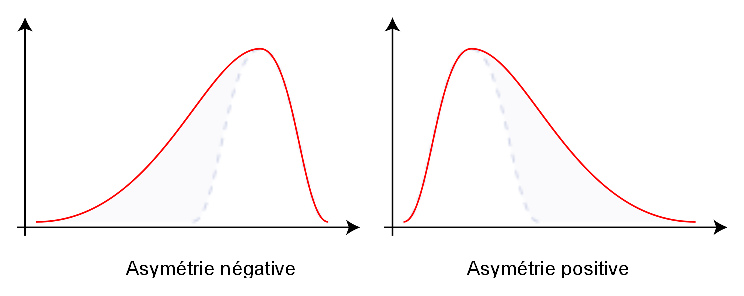
\includegraphics[scale=0.9]{images/skew.eps}
%	\end{center}
%	\scriptsize{Par Rodolfo Hermans (en.wikipedia)}
%}
%\frame{
%	\frametitle{Moments factoriels}
%	\pause
%	\begin{block}{Definition}
%		Soit $X$ une v.a., et soit $n\in\N$. Si $\mu_X=\Es{X}$, le nombre 
%		\[\Es{X(X-1)(X-2)\cdot\ldots\cdot(X-(n-1)}\] s'appelle le \defi{$n^\text{e}$ moment fatoriel de la v.a. $X$}.\\
%	\end{block}
%	Remarque : Le premier moment factoriel d'une v.a. est égal au premier moment par rapport à l'origine.\\
%}

\section[Var. et écart-type]{Variance et écart-type d'une v.a.}
\begin{frame}{Variance}
	\pause
	\begin{defn}{}
		Soit $X$ une v.a. dont l'espérance est $\mu_X$. Supposons que $p$ soit la fonction de masse de $X$ si $X$ est une v.a. discrète, ou que $f$ soit la densité de $X$ si elle est absolument continue. La variance de $X$, notée $\Var{X}$, est définie par
		\[\Var{X}=\begin{cases}
			\sum_{x\in\R}(x-\mu_X)^2\,p(x)&\quad \text{(cas discret),}\\
			\int_{-\infty}^{\infty}(x-\mu_X)^2\,f(x)dx&\quad \text{(cas absolument continu).}\end{cases}\]
	\end{defn}
\end{frame}
\begin{frame}{Outils de calcul}
	\begin{rem}
	On écrit parfois $V(X)$ ou $V[X]$ pour désigner la variance de $X$.
	\end{rem}
	\begin{thm}
		Soit $X$ une v.a., et soit $a$ et $b$ des nombres réels. Alors
		\begin{enumerate}
			\item \(\Var{X}=\Es{X^2}-\Es{X}^2\);\\
			\item \(\Var{aX+b}=a^2\Var{X}\).\\
		\end{enumerate}
	\end{thm}
\end{frame}
\begin{frame}{Écart-type et écart absolu moyen}
	\pause
	\begin{defns}
		\begin{itemize}
		\item Soit $X$ une v.a. dont la variance est \(\Var{X}\). L'écart-type de $X$, noté $\sigma_X$, est défini par
		\[\sigma_X=\sqrt{\Var{X}}.\]
		\item Soit $X$ une v.a. dont l'espérance est \(\mu_X\). L'écart absolu moyen de $X$, noté $\delta_X$, est défini par
		\[\delta_X=\Es{\left|X-\mu_X\right|}.\]
		\end{itemize}
	\end{defns}
\end{frame}
%\frame{
%	\frametitle{L'espérance --- cas général}
%	\pause
%	\begin{thm}{}
%		Soit $X$ une v.a. dont la fonction de répartition est $F_X(x)$. Supposons qu'au moins une des deux intégrales ci-dessous converge. Alors
%		\[\Es{X}=\int_{0}^{\infty}\left(1-F_X(x)\right)dx-\int_{-\infty}^{0}F_X(x)dx.\]
%	\end{thm}
%}
%\begin{frame}
%\begin{coro}{}
%		Dans le cas où $X$ prend des valeurs non négatives, nous avons que 
%		\[\Es{X}=\int_{0}^{\infty}\left(1-F_X(x)\right)dx=\int_{0}^{\infty}\P{X>x}dx.\]
%	\end{coro}
%	\begin{coro}{}
%		Dans le cas où $X$ est discrète et prend des valeurs non négatives, nous avons que 
%		\[\Es{X}=\int_{0}^{\infty}\P{X>x}dx=\sum_{k=0}^{\infty}\P{X>k}=\sum_{n=1}^{\infty}\P{X\geq n}.\]
%	\end{coro}
%\end{frame}
%\section[Approx. des moments]{Approximations des moments}
%\frame{
%	\frametitle{Approximation pour $\Es{g(X)}$}
%	\pause
%	\begin{block}{Proposition}
%		Soit $X$ une v.a. dont l'espérance est \(\mu_X\). Si $g$ est une fonction dérivable deux fois, alors on peut approximer $\Es{g(X)}$ à l'aide de l'équation
%		\[\Es{g(X)}\approx g(\mu_X)+\frac{1}{2}g''(\mu_X)\sigma_X^2.\]
%	\end{block}
%	
%}
%\frame{
%	\frametitle{Approximation pour $\Var{g(X)}$}
%	\pause
%	\begin{block}{Proposition}
%		Soit $X$ une v.a. dont l'espérance est \(\mu_X\), et la variance \(\sigma_X^2\). Si $g$ est une fonction dérivable, alors on peut approximer $\Var{g(X)}$ à l'aide de l'équation
%		\[\Var{g(X)}\approx \left(g'(\mu_X)\right)^2\sigma_X^2.\]
%	\end{block}
%}
%\section[f.g.m.]{Fonction génératrice des moments}
%\frame{
%	\frametitle{Définition de la fonction génératrice des moments}
%	\pause
%	\begin{block}{Définition}
%		La fonction génératrice des moments d'une v.a. $X$ est la fonction définie par \[M(t)=\Es{\text{e}^{tX}}.\]
%	\end{block}
%	Ainsi, nous avons que
%	\[M(t)=\begin{cases}
%		\sum_{x\in\R}\text{e}^{tx}\,p(x)&\quad \text{(cas discret),}\\
%		\int_{-\infty}^{\infty}\text{e}^{tx}f(x)\,dx&\quad \text{(cas absolument continu).}\end{cases}\]
%	On utilise l'abréviation fgm pour parler de la fonction génératrice des moments.
%}
%\frame{
%	\frametitle{Propriétés}
%	\pause
%	\begin{block}{Définition}
%		On dit que la fgm $M(t)$ est finie autour de l'origine s'il existe $t_0>0$ tel que $M(t)<\infty$ pour tout $t\in\intoo{-t_0}{t_0}$.
%	\end{block}
%	\begin{enumerate}
%		\item $0<M(t)\leq\infty\forall t\in\R$;\\
%		\item $M(0)=1$;\\
%		\item Si $X$ et $Y$ sont deux v.a. possédant la même fgm, et si la fgm est \defi{finie autour de l'origine}, alors $X$ et $Y$ possèdent la même distribution;\\
%		\item Si $X$ possède une fgm $M(t)$ finie autour de l'origine, alors toutes les dérivées de $M$ existent, sont finies, et sont continues autour de l'origine. De plus, pour tout $n\in\N$, on a que
%		\[\Es{X^n}=\frac{d^n}{dt^n}M(t)\vert_{t=0}.\]
%	\end{enumerate}
%}

\begin{frame}{Remarques}

 \begin{rems}
 	\begin{itemize}
 		\item Ce document est rédigé avec Beamer, une classe de \LaTeX.
 	\end{itemize}
 \end{rems}

 	\vfill
 	\footnotesize Pour signaler une erreur dans ce document, veuillez écrire à~\href{mailto:jerome.soucy@mat.ulaval.ca}{jerome.soucy@mat.ulaval.ca}.
 \end{frame}
\end{document}